\documentclass[11pt, letterpaper]{article}

% --- Essential Packages ---
\usepackage[utf8]{inputenc}
\usepackage[margin=1in]{geometry}
\usepackage{amsmath, amssymb, amsthm}  % amsmath for matrices and vectors
\usepackage{graphicx}
\usepackage{hyperref}
\usepackage{listings}                   % for showing code
\usepackage{xcolor}                     % for showing custom colours in code
\usepackage{float}                      % for adding [H] to figures, making them stay in place
\usepackage{booktabs}                   % for table lines

% Custom colours for code files
\definecolor{background}{RGB}{245, 245, 245} % Light grey background

\begin{document}

% --- Custom Single Title Page ---
\begin{titlepage}
  \centering
  \vspace*{0.5in}

  \begin{figure}[H]
    \centering
    \includegraphics[width=0.3\textwidth]{"../common/figures/University_of_Waterloo_seal.png"}
  \end{figure}

  \vspace{1.5cm}

  % Custom Title & Subtitle
  {\Huge \bfseries Lab 3: Design of the Outer Loop Controller \par}

  \vspace{0.5cm}
  {\Large MTE 484: Digital Control Systems \par}
  \vspace{0.1cm}
  {\Large Instructor Sergio Livera \par}
  \vspace{0.5cm}
  {\large Department of Mechatronics and Mechanical Engineering \par}



  \vfill % Automatically fills vertical space, pushing author/date to the bottom

  % Custom Author Info
  {\Large \textbf{Levi Rogalla} \par}
  {\Large \textbf{Alex Veric} \par}

  \vspace{1.5cm}

  {\large \today \par}

  \vspace*{0.5in}
\end{titlepage}

\clearpage
\thispagestyle{empty}
\begin{center}
  \vspace*{\fill}
  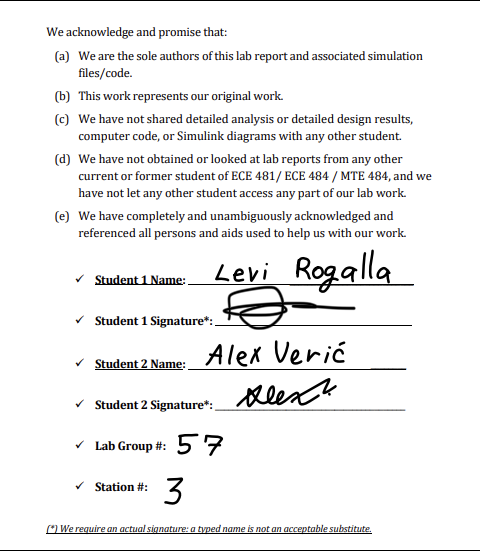
\includegraphics[width=\textwidth,height=0.9\textheight,keepaspectratio]{../common/figures/declaration.png}
  \vspace*{\fill}
\end{center}
\clearpage

\section{Question A}

Contrasting the last two lab reports, this report will focus on the outer loop of the system and its controller,
which controls the position of the ball on the beam, with feedback from the position sensor. The controller will
be first implemented in MatLab, building on the same model from the previous lab. The inner loop from last lab
involved a controller which decided how much voltage to input to the motor to get a desired motor angle, with
feedback from the motor position sensor. This can be seen below in Figure \ref{fig:a-lab2-matlab-model}.

\begin{figure}[H]
  \centering
  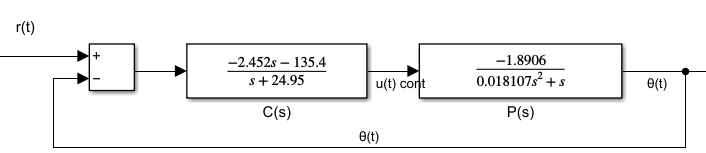
\includegraphics[width=0.7\textwidth]{figures/a-lab2-matlab-model.png}
  \caption{Lab 2 inner loop MatLab model}
  \label{fig:a-lab2-matlab-model}
\end{figure}

The output of the inner loop from Lab 2 is the current angle of the motor. However, the outer loop controller,
which will be the focus of this lab, takes the ball position (more specifically, the error between the desired and
current ball positions) as input. For this reason, we must use the values provided and determined in the previous lab
which allowed for the conversion between the motor angle, the beam angle, and finally the ball position. Below are
the transfer functions for each of the aforementioned conversions:

\begin{equation}
  \frac{\Phi(s)}{\Theta(s)} = K_2
\end{equation}

\begin{equation}
  \frac{Y(s)}{\Phi(s)} = \frac{K_3}{s^2}
\end{equation}

Where $\Theta (s)$ is the motor angle, $\Phi (s)$ is the beam angle, and $Y(s)$ is the position of the ball on the beam.
$K_2$ was given by the lab manual to be $K_2 = 0.0609$. $K_3$ was determined through experimentation with the
real system to be $K_3 = -0.14484227$, but this was deemed to be an unfit value, and so the approximation given by the
lab instructor, $K_3 = -4.25$, was used. These conversions were implemented in the MatLab inner loop model, as seen in figure
\ref{fig:a-inner-loop-model}, in order to obtain an inner loop system with ball position as its output.

\begin{figure}[H]
  \centering
  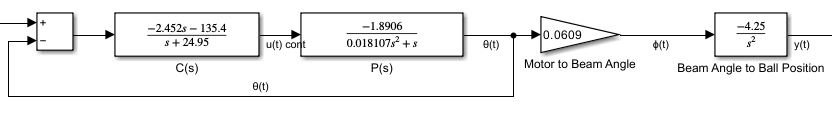
\includegraphics[width=0.7\textwidth]{figures/a-inner-loop-model.png}
  \caption{Updated inner loop model, with ball position as its output}
  \label{fig:a-inner-loop-model}
\end{figure}

An outer loop sample controller is given in the lab manual, as seen in equation \ref{eq:a-cont-sample-controller}, which is what will be used for the initial
tests of the outer loop system. The entire system model is shown in figure \ref{fig:a-system-model-sample-ctrler}.

\begin{equation}
  \label{eq:a-cont-sample-controller}
  C(s) = -7 \frac{s+0.35}{s+2.5}
\end{equation}

\begin{figure}[H]
  \centering
  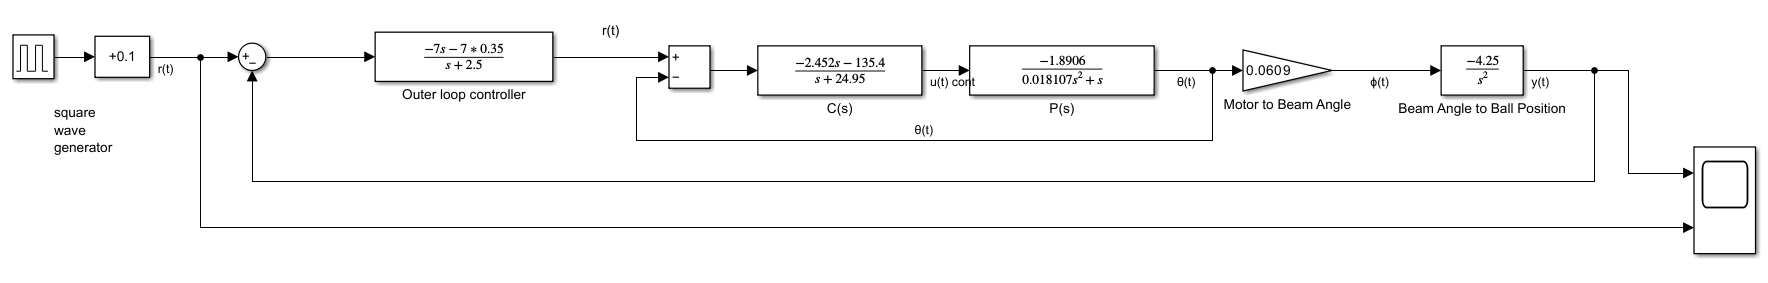
\includegraphics[width=0.7\textwidth]{figures/a-system-model-sample-ctrler.png}
  \caption{System model with sample outer loop controller}
  \label{fig:a-system-model-sample-ctrler}
\end{figure}

In figure \ref{fig:a-system-model-sample-ctrler-performance}, the system reacts to a square wave input, alternating
between $0.10$ and $0.25$ in a $50s$ period with a 50\% duty cycle. The $50s$ period was chosen because
it gave the model ample time to settle.

\begin{figure}[H]
  \centering
  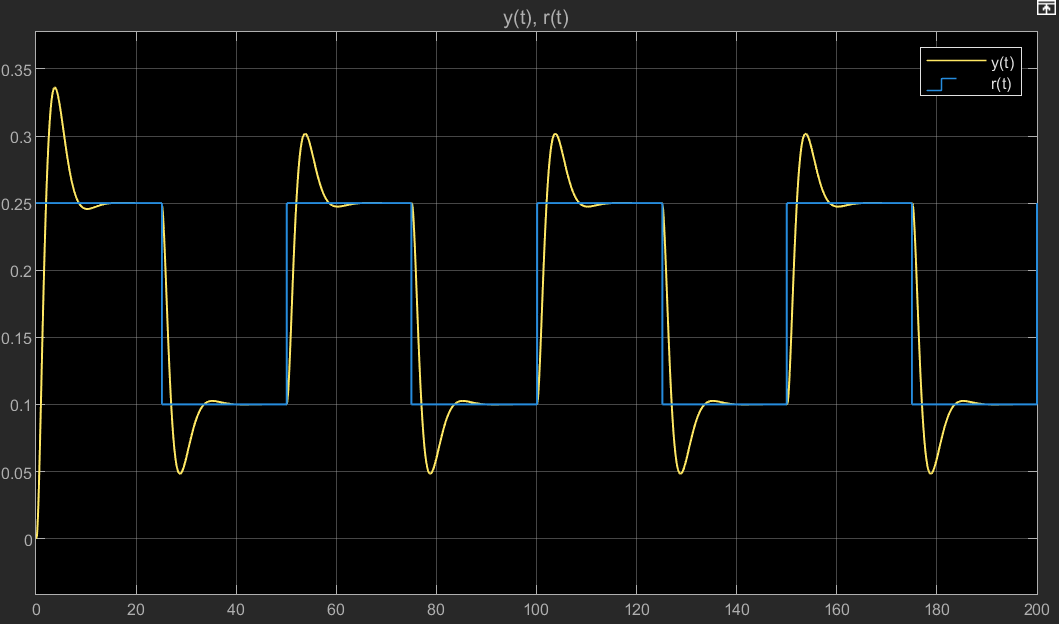
\includegraphics[width=0.7\textwidth]{figures/a-system-model-sample-ctrler-performance.png}
  \caption{System model performance to square wave generator with sample controller}
  \label{fig:a-system-model-sample-ctrler-performance}
\end{figure}

Figure \ref{fig:a-system-model-sample-ctrler-performance-zoomed} shows a closer look at the performance of a single
period.

\begin{figure}[H]
  \centering
  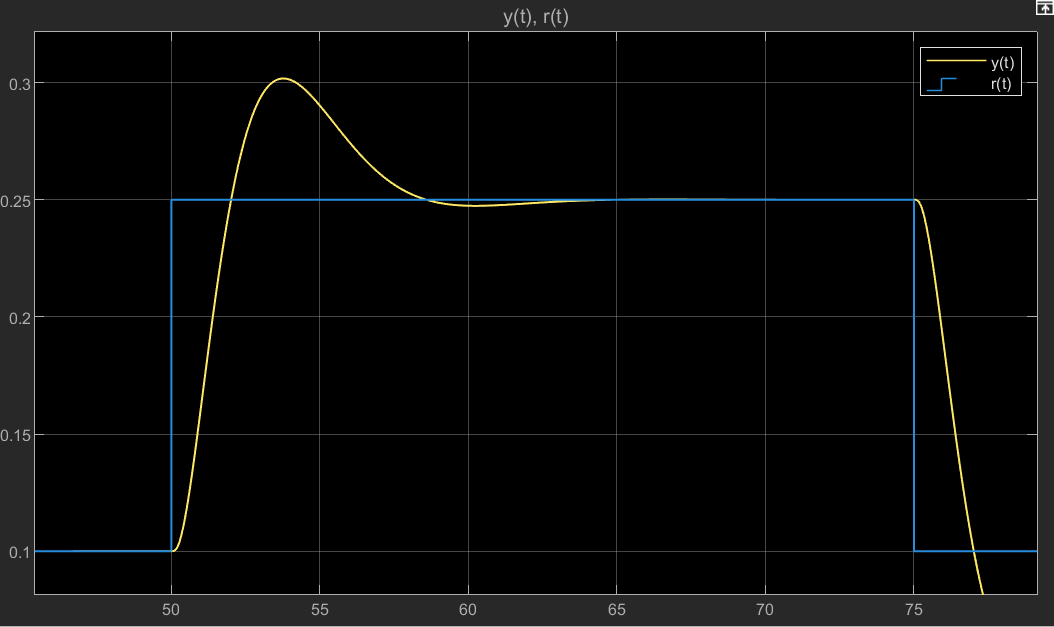
\includegraphics[width=0.7\textwidth]{figures/a-system-model-sample-ctrler-performance-zoomed.png}
  \caption{System model performance to square wave generator with sample controller, one period zoomed}
  \label{fig:a-system-model-sample-ctrler-performance-zoomed}
\end{figure}

\section{Question B}
The sample controller must not be implemented in the physical system. Since the controller is running on
an Arduino, which is digital, it must first be discretized. The Bilinear Transformation will be used,
with the following substitution for $s$:

\begin{equation}
  \label{eq:b-bilinear-transform}
  s = \frac{2}{T}\frac{z+1}{z-1}
\end{equation}

Where $T$ is the sampling period. This will be $T = 0.0005s$ which correlates to a sampling frequency of $2 kHz$;
these were the sampling time scales used in Lab 2, and so they will be reused. Equation \ref{eq:b-bilinear-transform}
was substituted into the equation for the continuous sample controller, equation \ref{eq:a-cont-sample-controller},
with $T = 0.0005s$ as the chosen sampling period, to get the following equation \ref{eq:b-disc-sample-controller}.

\begin{equation}
  \label{eq:b-disc-sample-controller}
  C[z] = \frac{-14.001225z + 13.998775}{2.00125z - 1.99875}
\end{equation}

The discrete controller now must be converted from the Z-domain into
the sampling domain using the inverse Z-transform. First, it is
reconfigured to be in terms of its input and output, $U[k]$ and $E[k]$:

\begin{equation}
  \frac{U[z]}{E[z]} = \frac{-14.001225z + 13.998775}{2.00125z - 1.99875}
\end{equation}

Then the Z-transform can be applied to convert it to the sampling domain:

\begin{equation}
  u[k] = 1.99875u[k - 1] - 14.001225e[k] + 13.998775e[k-1]
\end{equation}



\end{document}